\documentclass[12pt,a4paper,english,utf8]{report}
\usepackage[utf8]{inputenc}
\usepackage{amssymb}
\usepackage{graphicx}
\usepackage{listings}
\usepackage{float}
\usepackage{color}
\usepackage{wrapfig}
\usepackage{makeidx}
\usepackage{hyperref}
\usepackage{fancyhdr}

\pagestyle{fancy}
\fancyhf{}
\fancyhead[L]{\small{Tutorial: Java-API to GermaNet}}
\cfoot{\thepage}
\fancypagestyle{plain}{
\fancyhead[L]{\small{Tutorial: Java-API to GermaNet}}
}
%\fancypagestyle{acknowledgements} { %
%\fancyfoot[L]{Acknowledgements go to Marie Hinrichs and Holger Wunsch for their valuable input on both the features and usability of this API.}
%\cfoot{}
%\renewcommand{\headrulewidth}{0pt}}
\renewcommand*\thesection{\arabic{chapter}.\arabic{section}}

\makeindex

\definecolor{lightgray}{rgb}{0.9,0.9,0.9}
 \lstset{
   basicstyle=\scriptsize\ttfamily,
   keywordstyle=\bfseries\ttfamily\color{orange},
   stringstyle=\color{green}\ttfamily,
   commentstyle=\color{middlegray}\ttfamily,
   backgroundcolor=\color{lightgray},
   emph={square}, 
   emphstyle=\color{blue}\texttt,
   emph={[2]root,base},
   emphstyle={[2]\color{yac}\texttt},
   showstringspaces=false,
   flexiblecolumns=false,
   tabsize=2,
   %numbers=left,
   %numberstyle=\tiny,
   numberblanklines=false,
   stepnumber=1,
   numbersep=10pt,
   xleftmargin=15pt
}

\begin{document}

\begin{titlepage}
\begin{flushleft}
{\large University of Tübingen\\
Department of General and Computational Linguistics
Wilhelmstr. 19, 72074 Tübingen, Germany}\\[4.5cm]
\end{flushleft}

\begin{center}
{\huge \bfseries Tutorial:\\[0.4cm]
Java-API to GermaNet}\\[1.0cm]
{\large Version 8.0 (April 17, 2013)}\\[10.0cm]
\end{center}

\begin{flushleft} \small
Contributions from (alphabetic order):\\
Agnia Barsukova, Verena Henrich, Marie Hinrichs, Holger Wunsch.
\end{flushleft}


\end{titlepage}

\tableofcontents
\newpage



\chapter{Introduction}
This tutorial is about the Java-API\footnote{Acknowledgements go to Marie Hinrichs and Holger Wunsch for their valuable input on both the features and usability of this API.} to GermaNet. After an introduction of GermaNet and the API, there is a short overview of the GermaNet XML files (all in subsections of this chapter). In sections \ref{tutorialStarts} through \ref{tutorialEnds}, the Java-API to GermaNet is introduced by an example tutorial. In sections \ref{snippetsStart} through \ref{snippetsEnd}, further methods are explained to finally give a complete overview of the API.



\section{Basics About GermaNet}
GermaNet\footnote{See \href{http://www.sfs.uni-tuebingen.de/GermaNet/}{the GermaNet homepage}} is a lexical semantic network that partitions the lexical space in a set of concepts that are interlinked with semantic relations. A semantic concept is modeled by a synset (short for \emph{synonymy set}) in GermaNet. A synset is a set of words (called \emph{lexical units}) where all the words are taken to have (almost) the same meaning. Thus a synset is a set-representation of the semantic relation of synonymy.

There are two types of semantic relations in GermaNet: conceptual relations and lexical relations. Conceptual relations hold between two semantic concepts or synsets. They include relations such as hypernymy, part-whole relations, entailment, or causation. Lexical relations hold between two individual lexical units. Antonymy, a pair of opposites, is an example of a lexical relation.



\section{Java-API to GermaNet}
The Java-API to GermaNet represents a programming interface, which means that it provides several methods for accessing GermaNet data. The API is located in package \texttt{de.tuebingen.uni.sfs.germanet.api}.

The main class named \texttt{GermaNet} serves as a starting point to the API. When a \texttt{GermaNet} object is constructed, data is loaded from the GermaNet XML sources. All synsets (class \texttt{Synset}) and lexical units (class \texttt{LexUnit}) can be obtained through this object, which in turn can be used to examine attributes or find semantic relations, among other things.

This API specifies high-level look-up access to GermaNet data. As it is intended to be a read-only resource, no methods to extend or modify data are provided. All classes and methods are described in the enclosed Java API documentation.

Within the Java-API, there is a GermaNet class that is a collection of German lexical units (\texttt{LexUnit}) organized into synsets (\texttt{Synset}). A \texttt{GermaNet} object provides methods for retrieving lists of \texttt{Synsets} or \texttt{LexUnits}, which can be filtered by word category, orthographic form, or some combination.

A \texttt{Synset} has a \texttt{WordCategory} (adj, nomen, verben), a \texttt{WordClass} (Substanz, Relation, Kontakt, etc.), and consists of one or more \texttt{LexUnits} and a paraphrase (represented as \texttt{Strings}). The list of \texttt{LexUnits} for a \texttt{Synset} is never empty. A \texttt{Synset} object provides methods for retrieving the word category, the paraphrase, and all lexical units as well as methods for retrieving lists of conceptually related synsets.

\begin{sloppypar}
A LexUnit consists of an orthographical form (\texttt{orthForms}, represented as a \texttt{String}) and has optionally an orthographical variant (\texttt{orthVar}), an old orthographical form (\texttt{oldOrthForm}) and an old orthographical variant (\texttt{oldOrthVar}). Furthermore, a \texttt{LexUnit} object can have \texttt{Examples} and \texttt{Frames}, and it has the following attributes: \texttt{sense (int)}, \texttt{source (String)}, \texttt{styleMarking (boolean)}, \texttt{artificial (boolean)}, and \texttt{namedEntity (boolean)}. A \texttt{LexUnit} object provides methods for retrieving any of its properties, as well as methods for retrieving lists of other \texttt{LexUnits} lexically related to it.
\end{sloppypar}

A \texttt{Frame} is simply a container for frame data (\texttt{String}).

An \texttt{Example} consists of text (\texttt{String}) and zero or more \texttt{Frames}.

A \texttt{ConRel} is a set of possible conceptual relations between \texttt{Synsets} (represented as an enum type). A \texttt{ConRel} object provides methods for checking if a particular String is a valid conceptual relation, and for determining if a relation is transitive or not.  The set consists of the following transitive and non-transitive relations:

\renewcommand{\labelenumi}{•}
\begin{enumerate}
	\item transitive relations: hypernymy, hyponymy, meronymy, holonymy;
	\item non-transitive relations:	entailment, entailed, causation, caused, association.
\end{enumerate}

A \texttt{LexRel} is a set of possible lexical relations between \texttt{LexUnits} (represented as an enum type). A \texttt{LexRel} object provides a method for checking if a particular String is a valid lexical relation. Since there is only one transitive lexical relation (synonymy), and no special processing is required by the API to retrieve synonyms, there is no distinction made between transitive and non-transitive lexical relations. The set consists of the following relations:

\begin{enumerate}
	\item synonymy;
	\item antonymy;
	\item pertainymy.
\end{enumerate}

A \texttt{WordCategory} is a set of possible word categories (represented as an enum type) and contains the values: adj, nomen, verben.

A \texttt{WordClass} is a set of possible word classes (represented as an enum type) and contains 38 values: Substanz, Relation, Kontakt, etc.



\section{GermaNet XML Files}
The XML files represent the GermaNet data. There are two types of XML files. One type represents all synsets with their lexical units and all other properties. The other type represents all relations, both conceptual and lexical relations.



\subsection{Synset Files}
The XML files contatin all synsets in separated files. These files are named \texttt{wordcategory.wordclass.xml}, e.g. \texttt{adj.Allgemein.xml}. Each synset starts with a synset tag and contatins at least one lexical unit (encoded with the tag \texttt{lexUnit}) with its properties and frames and examples.

\begin{lstlisting}
<synsets>
  <synset id="s[0-9]" wordCategory="{adj|nomen|verben}">
    <lexUnit id="l[0-9]" sense="[0-9]" source="STRING"
     namedEntity="{yes|no}" artificial="{yes|no}" styleMarking="{yes|no}">
      <orthForm>STRING</orthForm>
      <orthVar>STRING</orthVar>
      <oldOrthForm>STRING</oldOrthForm>
      <oldOrthVar>STRING</oldOrthVar>
      <example><text>STRING</text><exframe>STRING</exframe></example>
      <frame>STRING</frame>
    </lexUnit>
    <paraphrase>STRING</paraphrase>
  </synset>
  ...
</synsets>
\end{lstlisting}



\subsection{Relation Files}
The relations are stored within a separate XML file. Both kinds of relations are encoded: conceptual (tag \texttt{con\_rel}) and lexical (tag \texttt{lex\_rel}) relations.

\begin{lstlisting}
<relations>
  <con_rel dir="{one|both|revert}" from="s[0-9]" to="s[0-9]"
       name="{has_hypernym|has_component_meronym|causes|is_related_to...}"
       inv="{has_hyponym|is_entailed_by|has_member_meronym...}"/>
  <lex_rel dir="{one|both|revert}" from="l[0-9]" to="l[0-9]"
       name="{has_antonym|has_pertainym|has_participle}"/>
  ...
</relations>
\end{lstlisting}





\chapter{Tutorial}
In this tutorial, we will develop a Java program that makes use of the most important part of the GermaNet-API. Once it is finished, your program will even be useful – it generates a description of a graph that shows a concept and all its hypernyms and hyponyms up to a certain distance from the concept, which is specified by the user. The file \emph{HypernymGraph.java} contains the source code for this tutorial, and is included in the GermaNet distribution.

The final output of the tutorial program will look somewhat like the graph in \ref{autograph}.

\begin{figure}[htb] 
	\begin{center}
		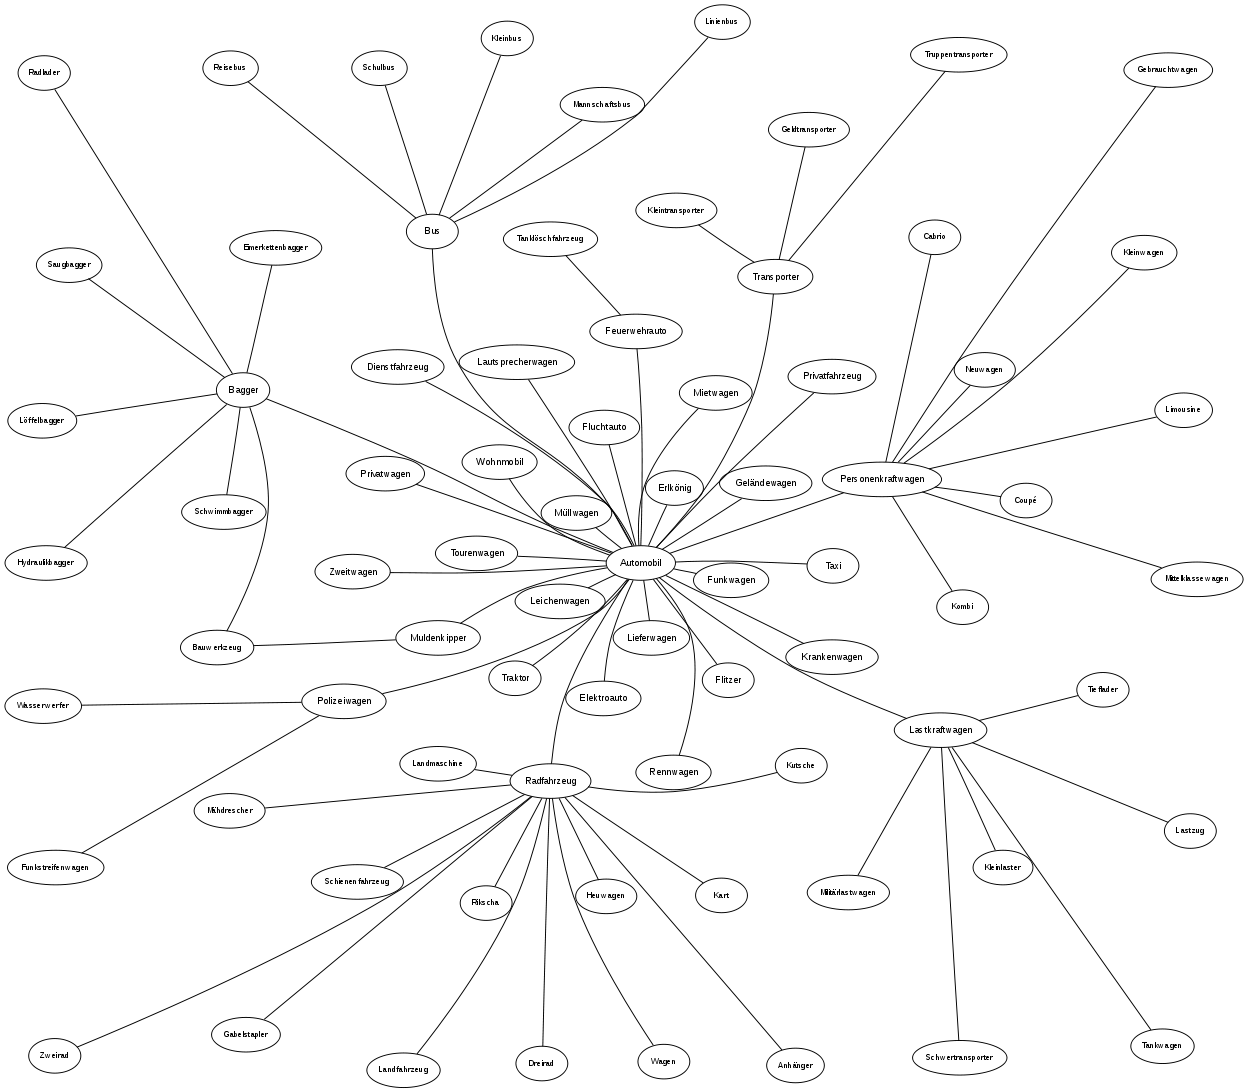
\includegraphics[scale=0.3]{auto_graph.png}
	\end{center}
	\caption{Output of this tutorial}
	\label{autograph}
\end{figure}

\section{Before You Start}
\label{tutorialStarts}
If you haven't done so already, you will need to obtain:

\renewcommand{\labelenumi}{\arabic{enumi}}
\begin{enumerate}
	\item The GermaNet data (either archived or unpacked to a directory typically named \emph{GN\_Vxx/GN\_Vxx\_XML}).
	\item The GermaNet Java library, called \emph{GermaNetApi8.0.jar}.
	\item In order to turn the graph description into an actual image, you will need the GraphViz Tools\footnote{The GraphViz Tools are freely available from \href{www.graphviz.org}{www.graphviz.org}}. Now would be a good time to download and install them.
\end{enumerate}

All of the classes described previously are defined in the package \\ \texttt{de.tuebingen.uni.sfs.germanet.api} within the \emph{GermaNetApi8.0.jar} file. You do not need to unpack the jar file.



\subsection{Classpath}
If you are working from the command line, you will need to add \\ \emph{GermaNetApi8.0.jar} to your CLASSPATH environment variable\footnote{See \href{http://faq.javaranch.com/java/HowToSetTheClasspath}{http://faq.javaranch.com/java/HowToSetTheClasspath} for help with setting your classpath on various operating systems.}.

If you are working within an IDE (such as NetBeans or Eclipse), add \emph{GermaNetApi8.0.jar} to the classpath for any project which uses GermaNet.



\subsection{Important Note on Memory}
Loading GermaNet requires more memory than the JVM allocates by default. Any application that loads GermaNet will most likely need to be run with JVM options that increase the memory allocated, like this:

\texttt{java -Xms128m -Xmx128m MyApplication}

These options can be added to your IDE's VM options so that they will be used automatically when your application is run from within the IDE.

Depending on the memory needs of the application itself, the 128's may need to be changed to a higher number. Be careful not to allocate too much memory for the JVM, though, as this may cause other running programs (like your windowing environment) to crash.



\section{Step 1: Importing Libraries}
Before we can create a \texttt{GermaNet} object, which loads the XML data and provides methods for looking up synsets and lexical units, we need to import the germanet library and several other necessary libraries.

The box below shows the first lines of the program. If you plan to type the program yourself along with the tutorial, create a file called \emph{HypernymGraph.java}.

\begin{lstlisting}
import de.tuebingen.uni.sfs.germanet.api.*;
import java.io.*;
import java.util.*;
public class HypernymGraph {
  public static void main(String[] args) {
    // to be filled in...
  }
}
\end{lstlisting}



\section{Step 2: Getting User Input}
The program needs some information to do its job that the user must supply:

\renewcommand{\labelenumi}{•}
\begin{enumerate}
	\item The word (i.e. orthographic form that represents a lexical unit) whose hypernyms and hyponyms should be displayed (to be accurate, it is not a lexical unit whose relations are to be displayed, but rather the synset that the lexical unit is a member of). In fact, a lexical unit could be a member of more than one synset if it is ambiguous, in which case the program will print the hypernyms and hyponyms for all of the synsets.
	\item The maximum distance up to which hypernyms and hyponyms are to be displayed.
	\item The name of the file to write the output to.
\end{enumerate}

\begin{lstlisting}
import de.tuebingen.uni.sfs.germanet.api.*;
import java.io.*;
import java.util.*;
public class HypernymGraph {
  public static void main(String[] args) {
    Scanner keyboard = new Scanner(System.in);
    String destName;
    File gnetDir;
    String word;
    int depth;
    Writer dest;
    System.out.println("HypernymGraph creates a GraphViz graph " +
            "description of hypernyms and hyponyms of a GermaNet" +
                "concept up to a given depth.");
    System.out.println("Enter <word> <depth> <outputFile> " +
                "[eg: Automobil 2 auto.dot]: ");
    word = keyboard.next();
    depth = keyboard.nextInt();
    destName = keyboard.nextLine().trim();
    // to be continued...
  }
}
\end{lstlisting}



\section{Step 3: Creating a GermaNet Object}
To construct a \texttt{GermaNet} object, provide the location of the GermaNet data. This can be done with a \texttt{String} representing the path to the directory containing the data, or with a \texttt{File} object. Generally speaking, file locations should never be hardcoded, but for the sake of simplicity, this code assumes that the GermaNet data files are in a directory called \\ \emph{/germanet/GN\_V80/GN\_V80\_XML}. Please change the line:

\begin{lstlisting}
gnetDir = new File("/germanet/GN_V80/GN_V80_XML");}
\end{lstlisting}

to reflect the actual location of the GermaNet data files on your computer.

\begin{lstlisting}
import de.tuebingen.uni.sfs.germanet.api.*;
import java.io.*;
import java.util.*;
public class HypernymGraph {
  public static void main(String[] args) {
    try {
      Scanner keyboard = new Scanner(System.in);
      String destName;
      String word;
      int depth;
      Writer dest;
      System.out.println("HypernymGraph creates a GraphViz graph " +
                  "description of hypernyms and hyponyms of a GermaNet" +
                  "concept up to a given depth.");
      System.out.println("Enter <word> <depth> <outputFile> " +
                  "[eg: Automobil 2 auto.dot]: ");
      word = keyboard.next();
      depth = keyboard.nextInt();
      destName = keyboard.nextLine().trim();
      gnetDir = new File("/germanet/GN_V80/GN_V80_XML");
      GermaNet gnet = new GermaNet(gnetDir);
	// to be continued...
    } catch (Exception ex) {
       ex.printStackTrace();
       System.exit(0);
    }
  }
}
\end{lstlisting}

Notice that we need to enclose the call to the constructor in a try/catch block. This is because the \texttt{GermaNet} object cannot be created if the data files are not found or are corrupted. If something goes wrong, an exception is thrown. We just print the stack trace and exit if this happens.



\section{Step 4: Finding All Synsets}
We can now find all the synsets in GermaNet that the word \texttt{orthForm} is a member of. Recall that words may be ambiguous, which means that a word (or lexical unit) may occur in more than one synset.

\begin{lstlisting}
      List<Synset> synsets;
      synsets = gnet.getSynsets(word);
      if (synsets.size() == 0) {
        System.out.println(word + " not found in GermaNet");
        System.exit(0);
      }
      // to be continued...
\end{lstlisting}

\begin{sloppypar}
The method \texttt{getSynsets(orthForm)}, which is defined in the class \texttt{GermaNet}, returns a \texttt{List} containing all of the \texttt{Synsets} that the word occurs in. If the size of this list is zero, then no synsets were found with a lexical unit containing the orthographic form \texttt{orthForm}, and we exit the program.
\end{sloppypar}

Each element of the \texttt{List synsets} is a \texttt{Synset} object. A \texttt{Synset} object has methods to retrieve all the lexical units that are members of the synset, and to find out about what other synsets are related to it with respect to a specific kind of conceptual relation. We will use some of the methods that are implemented in the \texttt{Synset} class in the next step.



\section{Step 5: Generating the Hypernym Graph}
We are now ready to generate the output, which is first stored in a \texttt{String} called \texttt{dotCode}, then written to the output file. As mentioned before, our program does not directly create images, but rather textual descriptions of graphs in the GraphViz graph definition language. These can later be turned into images using the GraphViz tools.

\begin{lstlisting}
      String dotCode = "";
      dotCode += "graph G {\n";
      dotCode += "overlap=false\n";
      dotCode += "splines=true\n";
      dotCode += "orientation=landscape\n";
      dotCode += "size=\"13,15\"\n";
      HashSet<Synset> visited = new HashSet<Synset>();
      for (Synset syn : synsets) {
        dotCode += printHypernyms(syn, depth, visited);
      }
      dotCode += "}";
      dest = new BufferedWriter(new OutputStreamWriter(
                      new FileOutputStream(new File(destName)), "UTF-8"));
      dest.write(dotCode);
      dest.close();

\end{lstlisting}

The first line of the \texttt{dotCode String} opens a GraphViz graph-statement. The following four lines then define the basic layout of the graph. Please refer to the GraphViz manual if you want to find out what exactly these statements do.

The algorithm that traverses the network to find the hypernyms and hyponyms is not very complicated. It works as follows:

\begin{enumerate}
	\item Start with a \texttt{Synset} that the lexical unit the user requested is a member of (called \texttt{Synset syn}). This becomes the center node of the graph.
	\item Look up all hypernyms of \texttt{syn} and add them to the graph as neighbor nodes of \texttt{syn}.
	\item Look up all hyponyms of \texttt{syn} and add them to the graph also.
	\item For each hypernym and hyponym found, recursively find and add their hypernyms and hyponyms to the graph, up to the maximum distance to the center node, as specified by the user.
\end{enumerate}

To sum up, the algorithm finds all hypernyms and hyponyms of a given \texttt{Synset syn}, adds them to the graph, and then in turn does exactly the same it did with syn with all of its hypernyms and hyponyms.

There is one catch, however, that we must pay attention to: Assume the algorithm looks at some \texttt{Synset s}. It finds all hypernyms of \texttt{s} and adds them to the graph. Then it recursively repeats all its steps for each hypernym \texttt{h} it found: That is, it first finds all hypernyms of \texttt{s}, then it finds all hyponyms of \texttt{h}. At this point, we must be careful, since the \texttt{Synset s} the algorithm looked at in the previous recursive step is, of course, a hyponym of \texttt{h}! We must make sure that the algorithm does not consider \texttt{Synsets} it already looked at over and over again. In our program, we use the \texttt{HashSet visited} for this: For each \texttt{Synset} the algorithm finds, we add the \texttt{Synset} to the visited set. Any \texttt{Synset} that is in the visited set is not considered any further by the algorithm in subsequent recursive steps.

The program proceeds by calling the static \texttt{printHypernyms()} method for each \texttt{Synset} in the \texttt{synsets} list. In the next step, we will turn to \texttt{printHypernyms()}, which is the implementation of the recursive algorithm sketched above.

We then finish up by adding a closing brace to the GraphViz description, write the code to the output file, and close the file.



\section{Step 6: Recursively Printing Hypernyms and Hyponyms}
The \texttt{printHypernyms()} method, which recursively adds all hypernyms and hyponyms of a synset to the hypernym graph, expects three arguments:

\begin{enumerate}
	\item The synset whose hypernyms and hyponyms are to be added next (the argument \texttt{synset})
	\item The remaining distance from the center node of the graph to the last hypernym or hyponym to be added (argument \texttt{depth})
	\item The set of synsets already visited (argument \texttt{visited})
\end{enumerate}

\begin{lstlisting}
static String printHypernyms(Synset synset, int depth,
                                HashSet<Synset> visited) {
\end{lstlisting}

Now declare the variables we will need later:

\begin{lstlisting}
    String rval = "";
    List<LexUnit> lexUnits;
    String orthForm = "";
    List<Synset> hypernyms = new ArrayList<Synset>();
    List<Synset> relations;
    String hypOrthForm;
    visited.add(synset);
    // to be continued...
  }
\end{lstlisting}

The synset is added to the \texttt{visited} set (to make sure the algorithm does not run in an infinite loop; see step 4).

We have already seen that the GermaNet-API contains a special class, \texttt{Synset}, that represents the properties of a synset. There is also a class \texttt{LexUnit} that represents the properties of a lexical unit. Both classes provide methods to obtain information about other objects in GermaNet the synset or lexical unit is related to. A lexical unit may contain multiple orthographic forms (i.e. \texttt{orthForm} (main orthographic form), \texttt{orthVar} (a variant of the main form), \texttt{oldOrthForm} (main orthographic form in the old German orthography), and \texttt{oldOrthVar} (a variant of the old form)), which represent different spellings of the same word. If there are several spellings of a word, for example \emph{Schloß} and \emph{Schloss} in the old and new German spelling, \emph{Schloss} represents \texttt{orthForm} and \emph{Schloß} represents \texttt{oldOrthForm}.

We will use the main orthographical form of the \texttt{LexUnit} that is first returned by \texttt{synset.getLexUnits()} as a representative for the concept the \texttt{Synset} represents. So we must first retrieve all lexical units that are a member of the synset:

\begin{lstlisting}
    lexUnits = synset.getLexUnits();
\end{lstlisting}

As you can see, this works very much the same as retrieving all lexical units in \texttt{GermaNet.getLexUnits()}: this method of the \texttt{Synset} class also returns a \texttt{List} of \texttt{LexUnit} objects.

We now fetch the first orthographic form of the first \texttt{LexUnit} and add it to the graph description, along with some formatting information:

\begin{lstlisting}
      orthForm = lexUnits.get(0).getOrthForm();
      rval += "\"" + orthForm + "\" [fontname=Helvetica,fontsize=10]\n";

\end{lstlisting}

Again, you can see that the way orthographic forms are retrieved is extremely similar to the way synsets and lexical units are accessed. Of course, since orthographic forms are plain strings, the \texttt{List} returned is of type \texttt{String}.

It is now time to collect all hypernyms and hyponyms and add them to the graph. Since we will make no difference in the graphical output between hypernyms and hyponyms we will store them (a little sloppily) in one list called hypernyms.

\begin{lstlisting}
     relations = synset.getRelatedSynsets(ConRel.has_hypernym);
     hypernyms.addAll(relations);
     relations = synset.getRelatedSynsets(ConRel.has_hyponym);
     hypernyms.addAll(relations);
\end{lstlisting}

\texttt{ConRel} is an \texttt{enum} class defined in GermaNet. Enums are special constructs in Java for storing constants. The \texttt{ConRel} class provides a way of telling the \texttt{getRelatedSynsets(conRel)} method which relation is being requested so that an invalid relation cannot be requested.

\texttt{ConRel.has\_hypernym} and \texttt{ConRel.has\_hyponym} are conceptual relations that apply between synsets. The complete list of conceptual realations are: hypernymy, hyponymy, meronymy, holonymy, entailment, entailed, causation, caused, and association.

Similarly, the \texttt{LexUnit} class contains a \texttt{getRelatedLexUnits(lexRel)} method which accepts a \texttt{LexRel} object as a parameter.

\begin{lstlisting}
01     for (Synset syn : hypernyms) { 
02       if (!visited.contains(syn)) { 
03         hypOrthForm = syn.getLexUnits().get(0).getOrthForm(); 
04         rval += "\"" + orthForm + "\" -- \"" + hypOrthForm + "\";\n"; 
05 
06         if (depth > 1) { 
07           rval += printHypernyms(syn, depth - 1, visited); 
08         } else { 
09           rval += "\"" + hypOrthForm + 
10                   "\"[fontname=Helvetica,fontsize=8]\n"; 
11         } 
12       } 
13     } 
14     // return the graph string generated 
15     return rval;
\end{lstlisting}

For each hypernym and hyponym we found, we first check if we have visited it before (line 2). If so, we skip it. Otherwise, we fetch the first orthographic form of the first lexical unit (line 3) and use it in line 4 to add an edge to the graph description between the node that represents the current synset and the node that represents the hypernym or hyponym (edges in GraphViz syntax are expressed by two node labels that are separated by --).

If the maximum distance to the center node has not yet been reached (line 6), we add the hypernyms and hyponyms of the current hypernym or hyponym by recursively calling \texttt{printHypernyms()} with a decremented depth. Otherwise, we add some formatting information for the hypernym or hyponym node.



\section{Step 7: Trying It Out}
\label{tutorialEnds}
This is it! We are now ready to test our program. Compile the source code using Java JDK 6.0 or above:

\texttt{javac HypernymGraph.java}

Then run the program:

\texttt{java -Xms256m -Xmx256m HypernymGraph}

Let's create a graph that shows the concept \emph{Automobil} in the center and the hypernyms and hyponyms up to a distance of two. When asked to enter the data, type: \texttt{Automobil 2 auto.dot}

\emph{HypernymGraph} creates a GraphViz graph description of hypernyms and hyponyms of a GermaNet concept up to a given depth.

\texttt{Enter <word> <depth> <outputFile> [eg: Automobil 2 auto.dot]:
Automobil 2 auto.dot}

This creates the graph description file \emph{auto.dot} in the current working directory. The first few lines should look like this:

\begin{lstlisting}
graph G {
overlap=false
splines=true
orientation=landscape
size="13,15"
"Automobil" [fontname=Helvetica,fontsize=10]
"Automobil" -- "Muldenkipper";
"Muldenkipper" [fontname=Helvetica,fontsize=10]
"Muldenkipper" -- "Bauwerkzeug";
"Bauwerkzeug" [fontname=Helvetica,fontsize=8]
"Automobil" -- "Bagger";
...
\end{lstlisting}

We can now use one of the GraphViz tools to create a visual representation of the graph from the graph description file in a PNG file called \emph{auto.png}:

\texttt{neato -Tpng auto.dot -o auto.png}

The GraphViz tools provide many more output formats and ways of influencing the layout of the graph, which are described in the GraphViz manuals\footnote{See \href{www.graphviz.org}{www.graphviz.org}}.

This finishes the tutorial. Please see the GermaNet javadoc documentation, viewable in your web browser, for a complete list of methods, including descriptions, available for each class within the germanet package.





\chapter{Code Snippets and Samples}
This chapter contains code snippets and samples that demonstrate how to use the GermaNet library objects and their methods.



\section{Creating a GermaNet Object}
\label{snippetsStart}
Before you can construct a \texttt{GermaNet} object, you need to make sure that the \emph{GermaNetApi8.0.jar} file is on your classpath, then import the library:

\begin{lstlisting}
import de.tuebingen.uni.sfs.germanet.api.*;
\end{lstlisting}

When a \texttt{GermaNet} object is created, it needs to know where to find the XML-formatted GermaNet data files. The location of the directory (or a .zip/.jar archive) containing the data files is sent as a parameter to the \texttt{GermaNet} constructor either as a \texttt{String} object:

\begin{lstlisting}
GermaNet gnet = new GermaNet("/germanet/GN_V80/GN_V80_XML/");
GermaNet gnet = new GermaNet("/germanet/GN_V80/GN_V80_XML.zip");
\end{lstlisting}

or a \texttt{File} object:

\begin{lstlisting}
File gnetDir = new File("/germanet/GN_V80/GN_V80_XML");
GermaNet gnet = new GermaNet(gnetDir);
\end{lstlisting}

To ignore case when getting \texttt{Synsets} and \texttt{LexUnits}, set the \texttt{ignoreCase} flag in the constructor:

\begin{lstlisting}
GermaNet gnet = new GermaNet("/germanet/GN_V80/GN_V80_XML/", true);
\end{lstlisting}

or:

\begin{lstlisting}
File gnetDir = new File("/germanet/GN_V80/GN_V80_XML");
GermaNet gnet = new GermaNet(gnetDir, true);
\end{lstlisting}

Unless otherwise stated in the javadoc documentation, all methods in all objects will return an empty \texttt{List} rather than \texttt{null} to indicate that no objects exist for a given request.



\section{Getting Synsets from a GermaNet Object}

A \texttt{Synset} has a \texttt{WordCategory} (i.e. adj, nomen, verben), a \texttt{WordClass} (Substanz, Relation, Kontakt, etc.), a paraphrase (represented as a \texttt{String}), and a \texttt{List} of \texttt{LexUnits}. The \texttt{List} of \texttt{LexUnits} for a \texttt{Synset} is never empty.
A \texttt{Synset} object provides methods for retrieving any of its properties as well as methods for retrieving \texttt{Lists} of other \texttt{Synsets} conceptually related to it. Once you have constructed a \texttt{GermaNet} object (called \texttt{gnet} in the examples below), you can retrieve \texttt{Lists} of \texttt{Synsets}, using orthographical form or word category filtering, if desired.
Get a \texttt{List} of all \texttt{Synsets}:

\begin{lstlisting}
List<Synset> allSynsets = gnet.getSynsets();
\end{lstlisting}

Get a \texttt{List} of all \texttt{Synsets} containing a lexical unit with \texttt{orthForm} \emph{Bank} (Note: if \texttt{gnet} was constructed with the \texttt{ignoreCase} flag set, then the following method call will return the same list with parameters such as \emph{bank, BANK} or \emph{BaNK}):

\begin{lstlisting}
List<Synset> synList = gnet.getSynsets("Bank");
\end{lstlisting}

Get a \texttt{List} of all \texttt{Synsets} which are adjectives (\texttt{WordCategory.adj}, other options are \texttt{WordCategory.nomen} and \texttt{WordCategory.verben}):

\begin{lstlisting}
List<Synset> adjSynsets = gnet.getSynsets(WordCategory.adj);
\end{lstlisting}

Get a \texttt{List} of all \texttt{Synsets} with word class Menge (\texttt{WordClass.Menge}):

\begin{lstlisting}
List<Synset> adjSynsets = gnet.getSynsets(WordClass.Menge);
\end{lstlisting}



\section{Working with Synsets}
Once you have obtained a \texttt{List} of \texttt{Synsets}, you can start processing them. A \texttt{Synset} object has methods for retrieving its word category, word class, lexical units (or just the orthographic forms of the lexical units), and paraphrases, as well as methods for retrieving synsets that are related to it.

To get a synset's word category and do further processing in case of an adjective:

\begin{lstlisting}
WordCategory wCat = aSynset.getWordCategory();
if (wCat == WordCategory.adj) {
    // do something
}
\end{lstlisting}

Or, similarly, check whether a synset belongs to a particular word class:

\begin{lstlisting}
WordClass wClass = aSynset.getWordClass();
if (wClass == WordClass.Allgemein) {
    // do something
}
\end{lstlisting}

Retrieving the paraphrase is done in a similar way:

\begin{lstlisting}
String paraphrase = aSynset.getParaphrase();
\end{lstlisting}

To get a synset's orthographic forms (retrieves a \texttt{List} of all orthographic forms in all the \texttt{LexUnits} that belong to this \texttt{Synset}):

\begin{lstlisting}
List<String> orthForms = aSynset.getAllOrthForms();
\end{lstlisting}

To get a list of all lexical units of a synset and iterate through them:

\begin{lstlisting}
List<LexUnit> lexList = aSynset.getLexUnits();
for (LexUnit lu : lexList) {
    // process lexical unit
}
\end{lstlisting}

Suppose you want to find all of the member meronyms of a synset:

\begin{lstlisting}
List<Synset> meronyms =
    aSynset.getRelatedSynsets(ConRel.has_member_meronym);
\end{lstlisting}

Sometimes you may have a conceptual relationship represented as a \texttt{String}. The following code can be used to validate the \texttt{String} and retrieve the relations:

\begin{lstlisting}
String aRel = "has_hypernym";
List<Synset> relList;
if (ConRel.isRel(aRel)) {// make sure aRel is a valid conceptual relation
    relList = aSynset.getRelatedSynsets(ConRel.valueOf(aRel));
}
\end{lstlisting}

The following are all valid calls to \texttt{getRelatedSynsets()}:

\begin{lstlisting}
aSynset.getRelatedSynsets(ConRel.has_hypernym);
aSynset.getRelatedSynsets(ConRel.has_hyponym);
aSynset.getRelatedSynsets(ConRel.has_component_meronymy);
aSynset.getRelatedSynsets(ConRel.has_component_holonymy);
aSynset.getRelatedSynsets(ConRel.has_member_meronymy);
aSynset.getRelatedSynsets(ConRel.has_member_holonymy);
aSynset.getRelatedSynsets(ConRel.has_substance_meronymy);
aSynset.getRelatedSynsets(ConRel.has_substance_holonymy);
aSynset.getRelatedSynsets(ConRel.has_portion_meronymy);
aSynset.getRelatedSynsets(ConRel.has_portion_holonymy);
aSynset.getRelatedSynsets(ConRel.is_related_to;
aSynset.getRelatedSynsets(ConRel.causes);
aSynset.getRelatedSynsets(ConRel.entails);
aSynset.getRelatedSynsets(ConRel.is_entailed_by); // and so on...
\end{lstlisting}

Suppose you are not interested in any particular relation, but want a \texttt{List} of all \texttt{Synsets} that are related to \texttt{aSynset} in any way:

\begin{lstlisting}
List<Synset> allRelations = aSynset.getRelatedSynsets();
\end{lstlisting}

For transitive relations (hypernymy, hyponymy, meronymy, holonymy), there is a method that retrieves a \texttt{List} of \texttt{Lists} of \texttt{Synsets}, where the \texttt{List} at position 0 contains the originating \texttt{Synset}, the \texttt{List} at position 1 contains the relations at depth 1, the \texttt{List} at position 2 contains the relations at depth 2, and so on up to the maximum depth. Using this data structure, some information cannot be included – namely, for any synset at depth n, you cannot determine which synset at depth n-1 it is a relation of. Nonetheless, you may find the method useful.

The following code prints the orthographic forms of each synset at every depth of the hyponyms of \emph{Decke}:

\begin{lstlisting}
List<List<Synset>> transHyponyms;
synList = gnet.getSynsets("Decke");
String spaces;
for (Synset s : synList) {
    spaces = "";
    transHyponyms = s.getTransRelatatedSynsets(ConRel.has_hyponym);
    for (List<Synset> listAtDepth : transHyponyms) {
        for (Synset synAtDepth : listAtDepth) {
            System.out.println(spaces + synAtDepth.getAllOrthForms());
        }
        spaces += "     ";
    }
}
\end{lstlisting}

Two \texttt{Synsets} are found containing the \texttt{orthForm} Decke. For each of them, we retrieve the hyponyms using the \texttt{getTransRelatedSynsets()} method, store the result in the \texttt{List} of \texttt{Lists} of \texttt{Synsets} called \texttt{transHyponyms}, and then print \texttt{transHyponyms}. The output looks like this: 

\begin{lstlisting}
[Decke]
     [Bettdecke]
     [Wolldecke]
     [Kuscheldecke]
     [Altardecke]
     [Satteldecke]
     [Plane]
     [Loeschdecke]
          [Plastikplane]
[Decke, Zimmerdecke]
     [Kuppel]
     [Beleuchtungsdecke]
     [Haengedecke]
     [Stuckdecke]
          [Zirkuskuppel]
\end{lstlisting}



\section{Getting LexUnits from a GermaNet Object}
A \texttt{LexUnit} may consist of multiple orthographic forms (stored as \texttt{Strings}), which represent different spellings of the same word:

\begin{enumerate}
	\item The main orthographic form \texttt{orthForm} (always set).
	\item A variant of the main form \texttt{orthVar} (optional).
	\item The main orthographic form in the old German orthography \texttt{oldOrthForm} (optional).
	\item A variant of the old form \texttt{oldOrthVar} (optional).
\end{enumerate}

If there are several spellings of a word, for example \emph{Schloß} and \emph{Schloss} in the old and new German spelling, \emph{Schloss} represents \texttt{orthForm} and \emph{Schloß} represents \texttt{oldOrthForm}.

\begin{sloppypar}
Lexical units can have \texttt{Frames} and \texttt{Examples}. Further attributes of a \texttt{LexUnit} are the following: \texttt{styleMarking (boolean), sense (int), orthVar (boolean), artificial (boolean), namedEntity (boolean)}, and \texttt{source (String)}. A \texttt{LexUnit} object provides methods for retrieving any of its properties, as well as methods for retrieving \texttt{Lists} of other \texttt{LexUnits} lexically related to it. Once you have constructed a \texttt{GermaNet} object (called \texttt{gnet} in the examples below), you can retrieve \texttt{Lists} of \texttt{LexUnits}, using orthographic form or word category filtering, if desired.
\end{sloppypar}

Get a List of all \texttt{LexUnits}:

\begin{lstlisting}
List<LexUnit> allLexUnits = gnet.getLexUnits();
\end{lstlisting}

Get a \texttt{List} of all \texttt{LexUnits} with \texttt{orthForm} \emph{Bank} (Note: if \texttt{gnet} was constructed with the \texttt{ignoreCase} flag set, then the following method call will return the same list with parameters such as \emph{bank, BANK} or \emph{BaNK}):

\begin{lstlisting}
List<LexUnit> lexList = gnet.getLexUnits("Bank");
\end{lstlisting}

\begin{sloppypar}
Get a \texttt{List} of all \texttt{LexUnits} which are nouns (\texttt{WordCategory.nomen}, other options are \texttt{WordCategory.adj} and \texttt{WordCategory.verben}):
\end{sloppypar}

\begin{lstlisting}
List<LexUnit> nomLexUnits = gnet.getLexUnits(WordCategory.nomen);
\end{lstlisting}



\section{Working with LexUnits}

\begin{sloppypar}
Once you have obtained a \texttt{List} of \texttt{LexUnits}, you can start processing them. A \texttt{LexUnit} object has methods for retrieving its \texttt{WordCategory, Synset}, orthographic forms (\texttt{orthForm, orthVar, oldOrthForm}, and \texttt{oldOrthVar}), and further attributes including word sense number \texttt{(sense), source, namedEntity, artificial}, and \texttt{styleMarking}, as well as methods for retrieving \texttt{LexUnits} that are lexically related to it.
\end{sloppypar}

To get the word category of a lexical unit and do further processing in case of a verb:

\begin{lstlisting}
WordCategory wCat = aLexUnit.getWordCategory();
if (wCat == WordCategory.verben) {
    // do something
}
\end{lstlisting}

To do the same for word class:

\begin{lstlisting}
WordClass wClass = aLexUnit.getWordClass();
if (wClass == WordClass.Geist) {
    // do something
}
\end{lstlisting}

To get the orthographic forms of a lexical unit:

\begin{lstlisting}
List<String> orthForms = aLexUnit.getOrthForms();
\end{lstlisting}

You may prefer to retrieve the main orthographic form:

\begin{lstlisting}
String orthForm = aLexUnit.getOrthForm();
\end{lstlisting}

You may prefer to just retrieve the variant of the main orthographic form:

\begin{lstlisting}
String orthVar = aLexUnit.getOrthVar();
\end{lstlisting}

To get the main orthographic form in the old German orthography:

\begin{lstlisting}
String oldOrthForm = aLexUnit.getOldOrthForm();
\end{lstlisting}

Retrieving the variant of the old orthographic form:

\begin{lstlisting}
String oldOrthVar = aLexUnit.getOldOrthVar();
\end{lstlisting}

Suppose you want to generate a \texttt{List} of \texttt{LexUnits} with word category \emph{nomen}, but you are not interested in named entities or artificial nouns. You could generate such a \texttt{List} with the following code (note that we use a real \texttt{Iterator} object here instead of just a simple for-loop because it is the only safe way to remove elements from a \texttt{List} while iterating):

\begin{lstlisting}
List<LexUnit> lexList = gnet.getLexUnits(WordCategory.nomen);
LexUnit aLexUnit;
Iterator<LexUnit> iter = lexList.iterator();
while (iter.hasNext()) {
    aLexUnit = iter.next();
    if (aLexUnit.isNamedEntity() || aLexUnit.isArtificial()) {
        iter.remove();
    }
}
// ... process lexList ...
\end{lstlisting}

Suppose you want to find all of the antonyms of a \texttt{LexUnit}:

\begin{lstlisting}
List<LexUnit> antonyms = aLexUnit.getRelatedLexUnits(LexRel.has_antonym);
\end{lstlisting}

Sometimes you may have a lexical relationship represented as a \texttt{String}. The following code can be used to validate the \texttt{String} and retrieve the relations:

\begin{lstlisting}String aRel = ”has_antonym”;
List<LexUnit> relList;
if (LexRel.isRel(aRel)) {// make sure aRel is a valid lexical relation
    relList = aLexUnit.getRelatedLexUnits(LexRel.valueOf(aRel));
}
\end{lstlisting}


The following are all valid calls to \texttt{getRelatedLexUnits()}:

\begin{lstlisting}
aLexUnit.getRelatedLexUnits(LexRel.has_synonym);
aLexUnit.getRelatedLexUnits(LexRel.has_antonym);
aLexUnit.getRelatedLexUnits(LexRel.has_pertainym); // and so on ...
\end{lstlisting}

Suppose you are not interested in any particular relation, but want a \texttt{List} of all \texttt{LexUnits} that are related to \texttt{aLexUnit} in any way:

\begin{lstlisting}
List<LexUnit> allRelations = aLexUnit.getRelatedLexUnits();
\end{lstlisting}

Finding the \texttt{Examples} and \texttt{Frames} is done as follows:

\begin{lstlisting}
List<Example> exList = aSynset.getExamples();
List<Frame> frameList = aSynset.getFrames();
\end{lstlisting}



\section{Working with Frames and Examples}
A \texttt{Frame} is simply a container for frame data, which can be retrieved with the \texttt{getData()} method. Frames occur in two contexts within GermaNet:

\renewcommand{\labelenumi}{\arabic{enumi}}
\begin{enumerate}
	\item A \texttt{List} of \texttt{Frames} may be present within a \texttt{Synset} object. You could print the \texttt{orthForms} of verb \texttt{Synsets} containing a \texttt{Frame} that begins with \emph{NN} like this:
	
\begin{lstlisting}
synList = gnet.getSynsets(WordClass.verben);
List<Frame> frameList;
boolean printIt;
for (Synset syn : synList) {
  printIt = false;
  frameList = syn.getFrames();
  for (Frame f : frameList) {
    if (f.getData().startsWith("NN")) {
      printIt = true;
    }
  }
  if (printIt) {
    System.out.println(syn.getAllOrthForms());
  }
}
\end{lstlisting}

\item A \texttt{List} of \texttt{Frames} may be present within an \texttt{Example} (which in turn is part of a \texttt{Synset}). We could print the \texttt{Examples} with \texttt{Frames} containing the substring \emph{AN} of verb \texttt{Synsets} with the following code:

\begin{lstlisting}
synList = gnet.getSynsets(WordClass.verben);
List<Example> exList;
List<Frame> frameList;
for (Synset syn : synList) {
  exList = syn.getExamples();
  for (Example ex : exList) {
    frameList = ex.getFrames();
    for (Frame f : frameList) {
      if (f.getData().contains("AN")) {
        System.out.println(f.getData() + " : " +ex.getText());
      }
    }
  }
}
\end{lstlisting}

\end{enumerate}



\section{Working with Interlingual Index (ILI) Data}
GermaNet-API 8.0 allows for working with the Interlingual Index data \footnote{\url{http://www.sfs.uni-tuebingen.de/lsd/ili.shtml}}, distributed with the GermaNet XML files. ILI links GermaNet synsets to English ones (originally, to Princeton WordNet 2.0) via several types of relations, such as synonymy, holonymy, meronymy etc. 

ILI data is automatically loaded along with the GermaNet XML data. You can then load \texttt{IliRecords} into a \texttt{List} by calling \texttt{getIliRecords()} metod on either a \texttt{LexUnit} or a \texttt{Synset}. 

\begin{lstlisting}
List<LexUnit> units = gnet.getLexUnits("abblocken");
for (LexUnit unit : units) {
  List<IliRecord> ili = unit.getIliRecords();
}
Synset ss = gnet.getSynsetByID(5711);
List<IliRecord> ili2 = ss.getIliRecords();
\end{lstlisting}

You can also get the complete \texttt{List} of all available \texttt{IliRecords} by calling \texttt{getIliRecords()} on the \texttt{GermaNet} object itself:

\begin{lstlisting}
List<IliRecord> allIlis = gnet.getIliRecords();
\end{lstlisting}

\texttt{IliRecord} object has methods for retrieving such attributes as the relation it has with a certain Princeton WordNet (PWN) synset (\texttt{ewnRelation}), the English word representing the PWN synset (\texttt{pwnWord}), as well as a list of all the synonyms belonging to it (\texttt{englishSynonyms}) and the corresponding English paraphrase (\texttt{pwn20paraphrase}), both from PWN 2.0. IDs from PWN 2.0 and PWN 3.0 are also available for most entries (\texttt{pwn20Id} and \texttt{pwn30Id}, respectively).

To get the relation of an \texttt{IliRecord} to the corresponding English synset:

\begin{lstlisting}
String ewnRelation = anIliRecord.getEwnRelation();
\end{lstlisting}

To retrieve the English word the index points to:

\begin{lstlisting}
String engWord = anIliRecord.getPwnWord();
\end{lstlisting}

Bear in mind that not all \texttt{IliRecords} have disambiguated links to particular English words, thus for some of them \texttt{getPwnWord()} method will return \texttt{null} values. All such \texttt{IliRecords} will have multiple synonymous words on the English side, which can be retrieved as follows:

\begin{lstlisting}
List<String> englishSynonyms = anIliRecord.getEnglishSynonyms();
\end{lstlisting}

Whenever English synset has only one word in it, the returned \texttt{List} will be empty, and the word in question will be retrievable by means of the \texttt{getPwnWord()} method.

To get English paraphrase for this \texttt{IliRecord}, use the following method:

\begin{lstlisting}
String paraphrase = anIliRecord.getPwn20paraphrase();
\end{lstlisting}


You may access the ID of the corresponding English synset from Princeton WordNet 2.0, or the ID from Princeton WordNet 3.0, if it's available (if it is not, ID is not \texttt{null} but rather represented as zeroes):

\begin{lstlisting}
String pwn20Id = anIliRecord.getPwn20Id();
String pwn30Id = anIliRecord.getPwn30Id();
\end{lstlisting}

Finally, if you're interested where a certain \texttt{IliRrecord} comes from (the original list developed in the framework of the EuroWordNet project, or one of the extensions created at the Tübingen University), try the following:

\begin{lstlisting}
String source = anIliRecord.getSource();
\end{lstlisting}



\section{Working with Wiktionary Paraphrases}
\label{snippetsEnd}
Another extention\footnote{\url{http://www.sfs.uni-tuebingen.de/lsd/wiktionary.shtml}} to GermaNet data (distributed alongside with the GermaNet XMLs), contains paraphrases, or definitions, for a part of the GermaNet \texttt{LexUnits} extracted from the German version of the free online lexicographical resource Wiktionary\footnote{See \href{http://de.wiktionary.org}{http://de.wiktionary.org}}.

You can retrieve a \texttt{List} of all the \texttt{WiktionaryParaphrases} for your \texttt{LexUnit} object:

\begin{lstlisting}
LexUnit unit = gnet.getLexUnitByID(3533);
List<WiktionaryParaphrase> wikis = unit.getWiktionaryParaphrases();
\end{lstlisting}

You can also get the complete \texttt{List} of all available \texttt{WiktionaryParaphrases} by calling \texttt{getWiktionaryParaphrases()} on the \texttt{GermaNet} object itself:

\begin{lstlisting}
List<WiktionaryParaphrase> wikis = gnet.getWiktionaryParaphrases();
\end{lstlisting}

\begin{sloppypar}
A \texttt{WiktionaryParaphrase} have methods for accessing its ID (\texttt{wiktionaryId}), the number of the Wiktionary sense (\texttt{wiktionarySenseId}), the paraphrase itself (\texttt{wiktionarySense}) and a boolean value indicating whether or not the paraphrase was taken from Wiktionary as is, or edited (\texttt{edited}).
\end{sloppypar}

To get the Wiktionary ID and sense ID, use:

\begin{lstlisting}
int wikiId = aWikiParaphrase.getWiktionaryId();
int senseId = aWikiParaphrase.getWiktionarySenseId();
\end{lstlisting}

You can retrieve the paraphrase itself:

\begin{lstlisting}
String wikiParaphrase =  aWikiParaphrase.getWiktionarySense();
\end{lstlisting}

Finally, to process the paraphrase only if it was edited, use the following: 

\begin{lstlisting}
if (aWikiParaphrase.hasBeenEdited()) {
    // do something 
}
\end{lstlisting}




\section{Working with Compounds}

GermaNet contains information about nominal compound splitting \footnote{\url{http://www.sfs.uni-tuebingen.de/lsd/compounds.shtml}}. Compounds are represented as modifier-head pairs, and some additional information can accompany the constituent parts. 

To access the available information on splitting of a compound, you can call \texttt{getCompoundInfo()} method on a \texttt{LexUnit}:

\begin{lstlisting}
LexUnit unit = gnet.getLexUnitByID(9559);
CompoundInfo compoundInfo =  unit.getCompoundInfo();
\end{lstlisting}

If the \texttt{LexUnit} in question is not a compound, or GermaNet has no information on the splitting, the \texttt{getCompoundInfo()} method will return \texttt{null}.

The \texttt{CompoundInfo} object gives you access to the information about compound modifier(s) and head. A compound has either one or two modifiers, the second option coming into play when it is unclear from which of the two words the compound has been derived.

\begin{lstlisting}
String modifier1 = compoundInfo.getModifier1();
String modifier2 = compoundInfo.getModifier2();
String head = compoundInfo.getHead();
\end{lstlisting}

Whereas heads of nominal compounds are always nouns, there is a great variation in modifier categories: adjectives (\texttt{CompoundCategory.Adjektiv}), nouns (\texttt{CompoundCategory.Nomen}), verbs (\texttt{CompoundCategory.Verb}), adverbs (\texttt{CompoundCategory.Adverb}), pronouns (\texttt{CompoundCategory.Pronomen}), particles (\texttt{CompoundCategory.Partikel}), and finally, prepositions \\ (\texttt{CompoundCategory.Präposition}) can all be compound modifiers. You may choose to work only with compounds which have adjectival modifiers:

\begin{lstlisting}
CompoundCategory modifier1Category = compoundInfo.getModifier1Category();
CompoundCategory modifier2Category = compoundInfo.getModifier2Category();
if (modifier1Category == CompoundCategory.Adjektiv ||
              modifier2Category == CompoundCategory.Adjektiv) {
    // do something
}
\end{lstlisting}

%\begin{sloppypar}
Both modifiers and heads can have certain properties associated with them. Modifier can be an abbreviation (\texttt{CompoundProperty.Abkürzung}), an affixoid (\texttt{CompoundProperty.Affixoid}), a konfix (\texttt{CompoundProperty.Konfix}), a foreign word (\texttt{CompoundProperty.Fremdwort}), an opaque morpheme \\ (\texttt{CompoundProperty.opaquesMorphem}), a personal name (\texttt{CompoundProperty.\\Eigenname}), or a word group (\texttt{CompoundProperty.Wortgruppe}). When a compound has two alternative modifiers, modifier property is \texttt{null}. Head can be an abbreviation, an affixoid, a foreign word, a konfix, an opaque morpheme, or a result of virtual formation (\texttt{CompoundProperty.virtuelleBildung}). To only work with compounds which include foreign words as modifiers or heads, you can use the following code:
%\end{sloppypar}

\begin{lstlisting}
CompoundProperty modifierProperty = compoundInfo.getModifierProperty();
CompoundProperty headProperty = compoundInfo.getHeadProperty();
if (modifierProperty == CompoundProperty.Fremdwort ||
              headProperty == CompoundProperty.Fremdwort) {
    // do something
}
\end{lstlisting}

\end{document}